\documentclass[12pt]{article}

\usepackage[margin=1in]{geometry}
\usepackage[bottom]{footmisc}
\usepackage{amsmath}
\usepackage{hyperref}
\usepackage{graphicx}
\usepackage{tikz}
\usepackage{pgfplots}
\usepackage{verbatim}

\hypersetup{
    colorlinks=true,
    linkcolor=blue,
    filecolor=magenta,      
    urlcolor=blue,
    }

\author{James O'Malley\\
Tufts University, EE104 Fall 2023\\
Medford, Massachusetts\\
james.o\_malley$@$tufts.edu\\
\underline{\href{https://github.com/jamesomalley/EE104}{https://github.com/jamesomalley/EE104}}}
\title{Probabilities around the Block: Analyzing Probability of Transaction Success for Various Blockchain Protocols\footnote{This paper is for informational purposes only. It is educational in nature and is not designed to be an offer or solicitation for the purchase or sale of any security, nor is it legal or tax advice. References to securities and strategies are for illustrative purposes only and do not constitute buy or sell recommendations. The information in this report should not be used as the basis for any investment decisions. At time of publishing, author held financial interest in Ethereum (ETH) and Polygon (MATIC) .}}
\date{December 12, 2022}


\begin{document}

\maketitle

\textbf{Abstract:} This paper analyzes the probability of a successful transaction occuring on a number of different blockchain protocols. Probability is measured over time to determine impact of major network upgrades on transaction success. It also explores the correlations between blockchain performance and price of the associated cryptocurrency tokens.\\

\textbf{Keywords:} blockchain, probability, bernoulli

%\footnote{fdsfd}
\pagebreak

\section{Introduction}

Though their associated cryptocurrency tokens are known by investors for volatile swings in price, the blockchain technology underlying these assets is intended to perform consistently regardless of price fluctuations [1]. A blockchain is a database of transactions that is updated and shared across many computers in a network [2]. 
An in-depth discussion of blockchain technology is outside the scope of this paper, however, blockchains generally allow users to transact on a publicy available ledger to transfer digital assets, execute smart contracts, or store data [2]. The Bitcoin blockchain is arguably the first and most popular blockchain, however, many competitive technologies, such as Ethereum, Solana and Avalanche, have arisen since the publication of the initial Bitcoin white paper in 2008 [3].   

Researchers have explored the probablistic nature of blockchains from a number of different angles, including the probablistic conditions of acheiving consensus on a blockchain, risk assessment using a blockchain protocol, network security using a probablistic model, and even a new method for validating transactions ("proof-of-probability")[5][6][7][8]. This paper will extend this research by comparing the probability of a successful transaction occurring across different blockchain protocols -- Bitcoin, Ethereum, Polygon, Solana, and Avalanche -- using data available from the protocols' public ledgers. 

While the exact mechanics of specific blockchain technologies vary by network, transcations on a blockchain are verified by other network participants and will succeed or fail for a variety of reasons. For example, transactions on the Ethereum network can fail due too low of computational cost allocated to the transaction by the user (referred to as "out of gas"), the transaction was reverted by one of the transaction's counterparties, bad instructions within the smart contract executing the transaction, or a token transfer failure (e.g. insufficient balance) [4].

This paper aims to compare the performance of various blockchain protocols by developing a model for the probability of transaction success and exploring statistical relationships betwen transaction success and asset price. It will begin by establishing a scope of analysis to identify which blockchain protocols are included in the analysis and how data is gathered. The next section will describe how probability can be applied to understanding blockchain transaction success. The remainder of the research will compare the probability of transaction success across the blockchain protocols in scope and measure the correlation between transaction success and the price of the cryptocurrency tokens associated with each blockchain.

\section{Analysis Scope}
The blockchains included in this research are listed in Table 2.1 below. Table 2.1 includes several metrics intended to measure the popularity of each blockchain:
\begin{itemize}
	\item Market capitalization: the total USD (\$) value of all tokens on the blockchain [12]
	\item Active addresses: number of unique addresses involved in a successful transaction as of November 30, 2022 [13] 
	\item Transactions: how many unique transactions (\emph{n}) were included in probability calculations \\
\end{itemize}
\textbf{Table 2.1}\\
\begin{tabular}{| c | c | c | c | c |}
\hline
\textbf{Name} & \textbf{Token} & \textbf{Market Cap}[10] & \textbf{Active Addresses}[13][14][15] & \textbf{Transactions}[11] \\
\hline
Bitcoin  & BTC & \$327.5B & 820K&773M\\
Ethereum & ETH & \$15B & 374K&1.8B\\
Solana & SOL & \$5.1B & 577K&26B\\
Avalanche & AVAX & \$4.2B & 38K& 208M \\
Polygon & MATIC & \$7.9B & 3K&2.3B\\
\hline
\end{tabular}\\
\\
\par Transaction data was accessed using Dune Analytics for Ethereum, Solana, Avalanche and Poloygon blockchains and Statoshi.info for Bitcoin [11][15]. Dune Analytics aggregates raw blockchain transaction data and stores it in a SQL accessible table for querying. Statoshi.info provides an interactive web application of Bitcoin transactions, including whether a transaction was accepted or rejected. 

While the date of the earliest transaction included in the analysis varies based on blockchain, all transaction data is through November 30, 2022.

More specifics of the underlying data collection and aggregation of this research paper, including the queries and datasets, can be found at \href{http://github.com/jamesomalley/EE104}{\underline{here}}.

\section{Applying Probability to Blockchain Transactions}
To help understand how probability applies to blockchain transactions, there are a few areas in which it helps to define equations which will be used in this research:
\begin{itemize}
	\item The probabilty (P[\emph{S}]) of a given transaction's success (\emph{s}=1) or failure (\emph{s}=0)
	\item Establishing an equation for calculating \emph{p} for each blockchain in totality and over time
	\item Measuring the correlation between blockchain transaction success/failure, total market capitalization and token price
\end{itemize}
For a given transaction, the probability of a success (\emph{S}) is a Bernoulli (\emph{p}) random variable. Bernoulli random variables apply to sequential experiments with independent trials in which each subexperiement has two possible outcomes[12]. Each attempted transaction can be considered a Bernoulli trial for which there is only two possible outcomes: success (\emph{s}=1) or failure (\emph{s}=0). 	

As a Bernoulli random variable, the probability mass function (PMF) of a successful blockchain transaction can be expressed as:
\[
P_{S}(\emph{s}) =
\begin{cases}
1-\emph{p}&\text{\emph{s} =0}\\
\emph{p}&\text{\emph{s}=1}\\
0&\text{otherwise}\\
\end{cases}
\]
where the parameter \emph{p} is in the range of 0$<\emph{p}<$1 [12].\\
To calculate \emph{p} for each individual blockchain transaction, \emph{t} = number of total successful transactions and \emph{n} = number of total attempted transactions. \emph{p} = P[\emph{S}] = \(\frac{t}{n}\). 

It is possible the probability of a successful transaction changes over time due to market fixes and technological changes such as an influx of new users more likely to make errors or upgrades to the blockchain technology by developers. As such, the probability of a successful transaction for any given month is P[\emph{S$_{i}$}] = \(\frac{t_{i}}{n_{i}}\) where \emph{i} denotes the month included in calculations. 

For the purposes of this research, the reliability of a blockchain will be measured by the expected value E[\emph{S}] (those with a higher E[\emph{S}] will be considered higher performing), and Var[\emph{S}] will be used to evaluate performance consistency. Expected value of S is E[\emph{S}] = $\mu_{S} = \sum \emph{sP(s)}.$ Variance is calculated as Var[\emph{S}] = $\sigma^{2}$= E[(\emph{S} - $\mu_{S})^2$].

The tokens associated with blockchain technologies (e.g. BTC for Bitcoin) are considered significant investment vehicles and, as such, it may be useful to understand whether a correlation exists between the performance of the underlying blockchain (i.e. probability of transaction success/failure) and the USD price of the associated token. The correlation coefficient is a normalized version of covariance that indicates the relationship of two random variables regardless of measurement units [12]. In this instance, the probability of a successful transaction (\emph{S}) will be measured as a percentage and token price (\emph{X}) will be measured in USD.

The correlation coefficient of these two random variables \emph{X} and \emph{S} is:
\[
\rho_{X,S} = \frac{Cov[\emph{X,S}]}{\sqrt{Var[\emph{X}]Var[\emph{Y}]}}=\frac{Cov[\emph{X,S}]}{\sigma_{X}\sigma_{S}}
\]

To calculate the covariance between asset price and the probability of transaction success, Cov[\emph{X,S}] = E[(\emph{X} - $\mu_{X})(\emph{S} - \mu_{S})$][12].

\section{Comparison of Blockchain Transaction Success Probabilities}
To analyze the probability of a successful transaction on each blockchain in scope of this research (P[\emph{S}]), individual blockchain transactions were quereied using Statoshi.info (Bitcoin) and Dune Analytics (all other blockchains) to measure values for \emph{t} and \emph{n} in order to calculate P[\emph{S}]. The results of this analysis can be found in Table 4.1 below.\\

\textbf{Table 4.1}\\
\begin{tabular}{| c | c | c | c | c | c |}
\hline
\textbf{Name} & \textbf{Date Range} & \textbf{\emph{t}} & \textbf{\emph{n}} & \textbf{\emph{p}} & \textbf{1-\emph{p}} \\
\hline
Ethereum & 10/1/17-11/30/22&1,681,731,602 &1,736,720,621 &0.968851&0.031149\\
Bitcoin  & 12/1/17-11/30/22&677,235,000 & 773,491,045&0.88 &0.12\\
Avalanche & 2/1/21-11/30/22&178,690,015 & 207,922,514& 0.859623&0.140377 \\
Polygon & 6/1/20-11/30/22&1,927,375,364 & 2,252,925,245 & 0.855499031&0.144500969\\
Solana & 10/1/20-11/30/22&20,754,207,378 & 26,561,603,366 & 0.781361241&0.218638759 \\
\hline
\end{tabular}\\
\\

From Table 4.1, it is observed that a transaction on the Ethereum blockchain has the greatest probability of success (0.968851) while a transaction on the Solana blockchain has the lowest success probability (0.781361241).
The blockchain industry is fast moving, however, and results may change over time as upgrades are made to the underlying technology or new users are onboarded to the networks. Figure 4.1 shows the value of P[\emph{S}] on a monthly basis since February 2021 (the earliest month for which data is available for all blockchains). \emph{i} = 0 for February 2021, \emph{i} = 1 for March 2021, etc.\\
\\
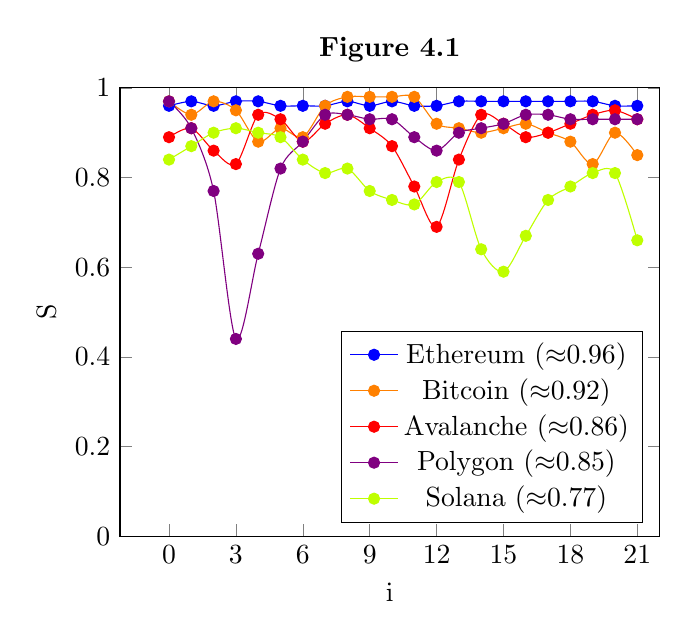
\begin{tikzpicture}
    \begin{axis}[
        title = {\textbf{Figure 4.1}},
	xlabel= i,
        ylabel= S,
        xmin=, xmax=22,
        ymin=0, ymax=1,
        xtick={0,3,6,9,12,15,18,21},
        ytick={0,.2,.4,.6,.8,1},
        legend pos =south east
        ]

    \addplot[smooth,color=blue,mark=*	]
        plot coordinates {
        (0,.96)
        (1,.97)
        (2,.96)
        (3, .97)
        (4, .97)
        (5,.96)
 (6, 0.96)
(7,0.96)
(8,.97)
(9,.96)
(10,.97)
(11,.96)
(12,.96)
(13,.97)
(14,.97)
(15,.97)
(16,.97)
(17,.97)
(18,.97)
(19,.97)
(20,.96)
(21,.96)
        };

    \addlegendentry{Ethereum ($\approx$0.96)}

\addplot[smooth,mark=*,orange] 
	plot coordinates {
        (0,.97)
        (1,.94)
        (2,.97)
        (3, .95)
        (4, .88)
        (5,.91)
 (6, 0.89)
(7,0.96)
(8,.98)
(9,.98)
(10,.98)
(11,.98)
(12,.92)
(13,.91)
(14,.9)
(15,.91)
(16,.92)
(17,.9)
(18,.88)
(19,.83)
(20,.9)
(21,.85)
    };
    \addlegendentry{Bitcoin ($\approx$0.92)}


    \addplot[smooth,color=red,mark=*	]
        plot coordinates {
        (0,.89)
        (1,.91)
        (2,.86)
        (3, .83)
        (4, .94)
        (5,.93)
 (6, 0.88)
(7,0.92)
(8,.94)
(9,.91)
(10,.87)
(11,.78)
(12,.69)
(13,.84)
(14,.94)
(15,.92)
(16,.89)
(17,.9)
(18,.92)
(19,.94)
(20,.95)
(21,.93)
        };
    \addlegendentry{Avalanche ($\approx$0.86)}

  \addplot[smooth,color=violet,mark=*	]
        plot coordinates {
        (0,.97)
        (1,.91)
        (2,.77)
        (3, .44)
        (4, .63)
        (5,.82)
 (6, 0.88)
(7,0.94)
(8,.94)
(9,.93)
(10,.93)
(11,.89)
(12,.86)
(13,.9)
(14,.91)
(15,.92)
(16,.94)
(17,.94)
(18,.93)
(19,.93)
(20,.93)
(21,.93)
        };
    \addlegendentry{Polygon ($\approx$0.85)}

  \addplot[smooth,color=lime,mark=*	]
        plot coordinates {
        (0,.84)
        (1,.87)
        (2,.9)
        (3, .91)
        (4, .9)
        (5,.89)
 (6, 0.84)
(7,0.81)
(8,.82)
(9,.77)
(10,.75)
(11,.74)
(12,.79)
(13,.79)
(14,.64)
(15,.59)
(16,.67)
(17,.75)
(18,.78)
(19,.81)
(20,.81)
(21,.66)
        };
    \addlegendentry{Solana ($\approx$0.77)}
    \end{axis}
    \end{tikzpicture}
\\
As indicated in Figure 4.1, the probability of transaction success for each blockchain does vary month-to-month and considering only more recent transactions does have some impact on results. Ethereum is both the best performing blockchain (with the highest E[\emph{S}] = 0.97) and the most consistently performing blockchain with a variance ($\sigma^{2}$)of $\approx$ 0.002. In contrast, Solana is the lowest performing blockchain overall with an E[\emph{S}] = 0.79 but is more consistent than Polygon with a variance of $\approx$ .0077 vs Polygon's variance of $\approx$ 0.0149. 

Polygon's higher variance appears to be a result of degraded performance from April to June 2021 which coincides with the onboarding of major decentralized finance protocols which may have influenced performance either due to new technology or new functionality [18].

Bitcoin's transaction success probability had the greatest change when considering only the more recent timeframes as depicted in Figure 4.1 The overall transaction success probability as measured in Table 4.1 is \emph{p} = 0.88, however, \emph{p} = 0.96 in the shorter timeframe. A major upgrade to the network, Taproot, went live in November 2021 and may have had  positive impact on the transaction probability success[19].

\section{Correlation Between Transaction Success and Asset Price}
In section 4, the probability of a successful blockchain transaction was established for each of the blockchains included in this research, including a month-over-month calculation of E[\emph{S}]. Many investors consider the cryptocurrency tokens associated with each blockchain technology as an investment asset class separate from stock markets, real estate and other traditional financial assets. A logical hypothesis is that a correlation exists between the performance of the blockchain technology and the value of its associated tokens.

Table 5.1 provides results of the the correlation coefficient of month-to-month P[\emph{S}] results and the closing price of the associated assets (the price on the last day of the month).\\

\textbf{Table 5.1}\\
\begin{tabular}{| c | c | c | c | c | c |}
\hline
\textbf{Name} & \textbf{E[\emph{S}]} & \textbf{E[\emph{X}]}[20] & \textbf{Cov[\emph{X,S}]} & \textbf{\emph{$\rho$}} \\
\hline
Ethereum/ETH & 0.96 & \$2,487.79 & 1.66 & $\approx$0.374 \\
Bitcoin/BTC  & 0.92 & \$38,562.95 & 231.67 & $\approx$0.395 \\
Avalanche/AVAX & 0.86 &\$44.25 & -0.84 & -.40268 \\
Polygon/MATIC & 0.85 &\$1.17 & -0.02 & -0.28673 \\
Solana/SOL & 0.77 & \$75.08 & -0.38 & -0.07 \\
\hline
\end{tabular}\\
\\

The results reflected in Table 5.1 appear to suggest that a correlation does not exist beteween the probability of blockchain transaction success and the prices of their associated cryptocurrency tokens. This suggests that the value investors place on the cryptocurrency tokens are associated with another market factor than transaction success of the underlying technology.

The calculated values for $\rho$ are never strong enough to suggest a relationship either postively or negatively (+/-.75) and do not agree in direction. Bitcoin and Ethereum have a moderately positive correlation between price and the probability of transaction success while the others are negative. 

\section{Conclusion}
This research established an approach for analyzing the probability of a successful transaction on the Avalanche, Bitcoin, Ethereum, Solana and Polygon blockchains as well as a method to correlate that probability to the prices of their associated cryptocurrency assets.

The analysis observed that difference do exist between each blockchain technology in terms of the probability that a given transaction will be successful, and that probability fluctuates over time. Significant changes in the probability of transaction success appear to coincide with major development milestones of the technology.

The analysis also measured whether a correlation exists between the probability of a transaction success and the price of cryptocurrency tokens. The results indicated that there is not a correlation between the two, and investors value the cryptocurrency tokens on other factors.

Blockchain technology represent a new method for peer-to-peer transactions on a public ledger. The wealth of data that these protocols generate provide ample opportunities for future research into users transact with each other.


\pagebreak
\section{Reference}
\begin{enumerate}
	\item Tyler Cowen. "Crypto's Values Comes From Crypto's Volatility." Bloomberg.com. https://www.bloomberg.com/opinion/articles/2022-06-02/how-should-we-value-crypto-by-how-volatile-crypto-assets-are, June 2, 2022 (accessed December 3, 2022)
	\item Ethereum Foundation. "What Is Ethereum? | ethereum.org" Ethereum.org. \\https://ethereum.org/en/what-is-ethereum/ (accessed December 3, 2022).
	\item Vinay Gupta. "A Brief History of Blockchain". Harvard Business Review. \\ https://hbr.org/2017/02/a-brief-history-of-blockchain (access December 3, 2022).
	\item Kaven Choi. "What are the Reasons for Failed Transactions?" Etherscan.io.\\ https://info.etherscan.com/reason-for-failed-transaction/ (accesssed December 3, 2022).
	\item Markinovic et al. "Probablistic Consensus of the Blockchain Protocol". \\ https://home.inf.unibe.ch/\~tstuder/papers/20190614\_probability\_blockchain.pdf 
	\item T. Salman, R. Jain and L. Gupta, "Probabilistic Blockchains: A Blockchain Paradigm for Collaborative Decision-Making," 2018 9th IEEE Annual Ubiquitous Computing, Electronics \& Mobile Communication Conference (UEMCON), 2018, pp. 457-465, doi: 10.1109/UEMCON.2018.8796512.
	\item K. Aiyar, M. N. Halgamuge and A. Mohammad, "Probability Distribution Model to Analyze the Trade-off between Scalability and Security of Sharding-Based Blockchain Networks," 2021 IEEE 18th Annual Consumer Communications \& Networking Conference (CCNC), 2021, pp. 1-6, doi: 10.1109/CCNC49032.2021.9369563.
	\item Kim, Sungmin \& Kim, Joongheon. (2018). POSTER: Mining with Proof-of-Probability in Blockchain. 841-843. 10.1145/3196494.3201592. 
     \item Shijie Zhang, Jong-Hyouk Lee, Analysis of the main consensus protocols of blockchain, ICT Express, Volume 6, Issue 2, 2020, Pages 93-97, ISSN 2405-9595, \\https://doi.org/10.1016/j.icte.2019.08.001. \\(https://www.sciencedirect.com/science/article/pii/S240595951930164X)
	\item CoinMarketCap, "Cryptocurrency Prices, Charts And Market Capitalizations | CoinMarketCap." https://coinmarketcap.com/ (accessed December 8, 2022).
	\item Dune Analytics AS. "Dune." Dune. https://dune.com/queries (accessed November, 2022)
	\item Yates, Roy D., and David J. Goodman. \emph{Probability and Stochastic Processes: a Friendly Introduction for Electrical and Computer Engeineers}. Third edition., John Wiley \& Sons, 2014.
	\item DST Systems, Inc. "Understanding Market Capitalization". https://www.fidelity.com/\\learning-center/trading-investing/fundamental-analysis/understanding-market-capitalization (accessed December 3, 2022).
	\item Glassnode. "Bitcoin: Active Addresses". https://studio.glassnode.com/metrics?a=BTC\&m=\\addresses.ActiveCount (accessed December 8, 2022).
	\item Statoshi.info. "Transactions - Grafana." https://statoshi.info/d/000000006/transactions?\\orgId=1\&from=now\%2Fy\&to=now (accessed December 8, 2022).
	\item Solscan. "Solana Analytics | Solscan." https://analytics.solscan.io/ (accessed December 8, 2022).
	\item Avalanche. "Avalanche (C-Chain)." https://subnets.avax.network/c-chain/stats?timespan999\\=ONE\_YEAR (accessed December 8, 2022).
	\item Polygon. "About Us | Polygon." https://polygon.technology/about (accessed December 12, 2022).
	\item Bitcoin.org. "Bitcoin Core 0.21.1 released" https://bitcoin.org/en/releases/0.21.1/ (accessed December 12, 2022).
	\item Yahoo. "Yahoo Finance  - Stock Market Live, Quotes, Business \& Finance News" https://finance.yahoo.com/ (accessed December 12, 2022).
\end{enumerate}
\end{document}
